%%
%% Beginning of file 'sample.tex'
%%
%% Modified 2015 December
%%
%% This is a sample manuscript marked up using the
%% AASTeX v6.x LaTeX 2e macros.

%% AASTeX is now based on Alexey Vikhlinin's emulateapj.cls 
%% (Copyright 2000-2015).  See the classfile for details.
%%
%% AASTeX requires revtex4-1.cls (http://publish.aps.org/revtex4/) and
%% other external packages (latexsym, graphicx, amssymb, longtable, and epsf).
%% All of these external packages should already be present in the modern TeX 
%% distributions.  If not they can also be obtained at www.ctan.org.

%% The first piece of markup in an AASTeX v6.x document is the \documentclass
%% command. LaTeX will ignore any data that comes before this command. The 
%% documentclass can take an optional argument to modify the output style.
%% The command below calls the preprint style  which will produce a tightly 
%% typeset, one-column, single-spaced document.  It is the default and thus
%% does not need to be explicitly stated.
%%

%% using aastex version 6
\documentclass[onecolumn]{aastex6}
\usepackage{subfigure}
\usepackage{amsmath}
\usepackage{graphicx}

%% The other main article choice is a tightly typeset, two-column article
%% that more closely resembles the final typeset pdf article.
%%
%% \documentclass[twocolumn]{aastex6}
%% 
%% There are other optional arguments one can envoke to allow other 
%% actions. 
%%
% These are the available options:
%   manuscript	: onecolumn, doublespace, 12pt fonts
%   preprint	: onecolumn, single space, 10pt fonts
%   preprint2	: twocolumn, single space, 10pt fonts
%   twocolumn	: a two column article. Probably not needed, but here just in case.
%   onecolumn	: a one column article; default option.
%   twocolappendix: make 2 column appendix
%   onecolappendix: make 1 column appendix is the default. 
%   astrosymb	: Loads Astrosymb font and define \astrocommands. 
%   tighten	: Makes baselineskip slightly smaller
%   times	: uses times font instead of the default
%   linenumbers	: turn on lineno package.
%   trackchanges : required to see the revision mark up and print output
%   numberedappendix: Labels appendix sections A, B, ... This is the default.
%   appendixfloats: Needed. Resets figure and table counters to zero

%% these can be used in any combination, e.g.
%%
%% \documentclass[twocolumn,twocolappendix,linenumbers,trackchanges]{aastex6}

%% If you want to create your own macros, you can do so
%% using \newcommand. Your macros should appear before
%% the \begin{document} command.
%%
\newcommand{\vdag}{(v)^\dagger}
\newcommand\aastex{AAS\TeX}
\newcommand\latex{La\TeX}

%% AASTeX 6.0 supports the ability to suppress the names and affiliations
%% of some authors and displaying them under a "collaboration" banner to
%% minimize the amount of author information that to be printed.  This 
%% should be reserved for articles with an extreme number of authors.
%%
%% Mark up commands to limit the number of authors on the front page.
\AuthorCallLimit=2
%% Will only show Schwarz & Muench since Schwarz and Muench
%% are in the same \author call. 
\fullcollaborationName{The Friends of AASTeX Collaboration}
%% will print the collaboration text after the shortened author list.
%% These commands have to COME BEFORE the \author calls.
%%
%% Note that all of these author will be shown in the published article.
%% This feature is meant to be used prior to acceptance to make the
%% front end of a long author article more manageable.
%% Use \allauthors at the manuscript end to show the full author list.

%% The following command can be used to set the latex table counters.  It
%% is needed in this document because it uses a mix of latex tabular and
%% AASTeX deluxetables.  In general it should not be needed.
%\setcounter{table}{1}

%%%%%%%%%%%%%%%%%%%%%%%%%%%%%%%%%%%%%%%%%%%%%%%%%%%%%%%%%%%%%%%%%%%%%%%%%%%%%%%%
%%
%% The following commented section outlines numerous optional output that
%% can be displayed in the front matter or as running meta-data.
%%
%% You can insert a short comment on the title page using the command below.
%% \slugcomment{Not to appear in Nonlearned J., 45.}
%%
%% If you wish, you may supply running head information, although
%% this information may be modified by the editorial offices.
%%\shorttitle{\aastex sample article}
%%\shortauthors{Schwarz et al.}
%%
%% You can add a light gray and diagonal water-mark to the first page 
%% with this command:
%% \watermark{text}
%% where "text", e.g. DRAFT, is the text to appear.  If the text is 
%% long you can control the water-mark size with:
%% \setwatermarkfontsize{dimension}
%% where dimension is any recognized LaTeX dimension, e.g. pt, in, etc.
%%
%%%%%%%%%%%%%%%%%%%%%%%%%%%%%%%%%%%%%%%%%%%%%%%%%%%%%%%%%%%%%%%%%%%%%%%%%%%%%%%%

%% This is the end of the preamble.  Indicate the beginning of the
%% paper itself with \begin{document}.

\begin{document}

%% LaTeX will automatically break titles if they run longer than
%% one line. However, you may use \\ to force a line break if
%% you desire.

\title{HW 07: Lab Techniques and Observation Planning}

%% Use \author, \affil, plus the \and command to format author and affiliation 
%% information.  If done correctly the peer review system will be able to
%% automatically put the author and affiliation information from the manuscript
%% and save the corresponding author the trouble of entering it by hand.
%%
%% The \affil should be used to document primary affiliations and the
%% \altaffil should be used for secondary affiliations, titles, or email.

%% Authors with the same affiliation can be grouped in a single
%% \author and \affil call.
\author{Bryan Yamashiro\altaffilmark{1},}
\author{Daichi Hiramatsu\altaffilmark{3},Gabrielle Melamed\altaffilmark{2},James Ou\altaffilmark{2}}


\affil{University of Hawaii at Manoa \\
2500 Campus Road \\
Honolulu, HI 96822}


%% Use the \and command so offset the last author.

%% Notice that each of these authors has alternate affiliations, which
%% are identified by the \altaffilmark after each name.  Specify alternate
%% affiliation information with \altaffiltext, with one command per each
%% affiliation.

\altaffiltext{1}{A cool dude}
\altaffiltext{2}{Another cool dude}


%% From the front matter, we move on to the body of the paper.
%% Sections are demarcated by \section and \subsection, respectively.
%% Observe the use of the LaTeX \label
%% command after the \subsection to give a symbolic KEY to the
%% subsection for cross-referencing in a \ref command.
%% You can use LaTeX's \ref and \label commands to keep track of
%% cross-references to sections, equations, tables, and figures.
%% That way, if you change the order of any elements, LaTeX will
%% automatically renumber them.

%% We recommend that authors also use the natbib \citep
%% and \citet commands to identify citations.  The citations are
%% tied to the reference list via symbolic KEYs. The KEY corresponds
%% to the KEY in the \bibitem in the reference list below. 

\section{Noise}
\begin{itemize}
\item{\underline{Thermal Noise\,(Darks)} - Noise contributed mainly by components\,(electronics) within the imager itself. Even with no light, pixels produce current and adds to the ambient flux.}
\item{\underline{Background} - Ambient regions that also include darks. Flux not from the target and intense regions, analogous to contamination not in the regions.}
\item{\underline{Flats} - Normalized field that accounts for pixel variation. Subtract darks and divide by median of the remainder.}
\item{\underline{Other sources of deviation} - Chosen wavelengths/filters, exposure time, bias\,(mainly only if exposure times are not identical)}
\end{itemize}

\section{Useful Numpy Functions}
\noindent np.mean() -- mean value\\
np.max() -- maximum value\\
np.min() -- minimum value\\
np.indices() -- indices of set parameters\,(can be (rows,columns))\\
np.log10() -- log base 10\\
np.shape() -- dimensions and shape of object\\
np.std() -- standard deviation\\
np.sum() -- total sum of defined\\
np.sqrt() -- square root


\section{Photometry}
Photometry is the measurement of an object brightness. Collecting measurements over a period shows the variation over time through magnitudes and subsequent light curves.


\noindent 1) Obtain data and header information from .fits files. Print statements are very important, use exit(0) to debug issues and to end code at that specific line. The header is first loaded with\,(hdulist = fits.open('filename.fits')). The header is then invoked by\,(hdulist.info()|header = hdulist[0].header|print header). Main data input reader is np.genfromtxt, refer to \url{https://docs.scipy.org/doc/numpy/reference/generated/numpy.genfromtxt.html}.
\\
2) Determine darks and backgrounds. This information is usually under the header, note that there may be multiple header inputs and specify with [0] or [1]. Useful information from the header includes read noise, background, gain, exposure time, etc. Note some headers do not include these information segments and must be derived. When using aperture photometry using a log10 of the background and color contours of the image allows for a first order approximation of the target/reference/background, for example\,(showIm = np.log10(background)|cbkg = plt.contourf(showIm,256)). A color bar can be added to the contour by\,(plt.colorbar(cbkg).set\_label(label='Contour Levels',size=16) \#,weight='bold').
\\
3) Aperture photometry, the scipy package\,(from astropy.coordinates import Angle
) is useful for RA/Dec conversions. RA: Angle('\#\#h\#\#m\#\#.\#\#s').deg and Dec: Angle('$\pm$\#\#d\#\#m\#\#.\#\#s').deg in degrees. A useful method included pinpointing a target and creating a box around it, for example\,(background\_aperture = image[dec\_conv\_bk-30:dec\_conv\_bk+30, ra\_conv\_bk-30:ra\_conv\_bk+30]). It is imperative to note that the coordinates may not be precise and a pinpoint location could be many pixels off. Therefore, using this technique, a check is to increase the aperture size to view objects near the literature coordinates.
\clearpage
\section{Relevant Equations}

\subsection{Image correction}

If corrected image isn't provided, the image must be normalized. The exposure times for each, equations\,\ref{correctedimage} and \ref{normflats}, must be the same respectively or a gain must be applied. The exposure time of equation\,\ref{normflats} isn't import when plugging into the corrected image equation because it is a ratio at that point.
\begin{equation}
\text{Corrected Image} = \frac{\text{Science Observation Image - Dark\,(same exp. time)}}{\text{Normalized Flat}}
\label{correctedimage}
\end{equation}

\begin{equation}
\text{Normalized Flat} = \frac{\text{flat - dark}}{\text{mean(flat - dark)}}
\label{normflats}
\end{equation}

\subsection{Aperture photometry}

Pixel variance\,(s$^2$) is noted in equation\,\ref{variance}. The equation includes the number of electrons\,(n) in the pixel\,(counts$\times$gain), the background\,(b) which again is\,(counts\*gain), dark level\,(d), and the read noise squared\,(r$^2$). There are cases where d and r$^2$ can be assumed to be zero.
\begin{equation}
s^2 = n+b+d+r
\label{variance}
\end{equation}

For bright sources n$>$d and the signal-to-noise ratio will be the square root of n\,(basically Poisson). The signal to noise ratio determines the total number of counts, which depends on stellar flux\,(N$_{rate}$) and integration time\,(t). 
\begin{equation}
\text{SNR} = \sqrt{N_{rate}}\sqrt{t}
\label{snr}
\end{equation}


The zero point is found through equation\,\ref{zp}. The respective flux and magnitudes are used for identical filters.
\begin{equation}
\text{Zero Point} = Magnitude\,[Band] + 2.5\log(Flux\,[Band]) - 2.5\log(exposure time)
\label{zp}
\end{equation}

\indent The flux of both J-star\,(F$_{\star}$) and J-standard\,(F$_{\dagger}$), provided in equation\,\ref{flux}, were obtained with background subtraction, while also taking the gain\,($\xi$) into account. The total counts of photons\,(N$_{\star,\dagger}$) from the star apertures were subtracted with the total background photon counts\,(B). B was determined by finding the sum of counts within the background aperture.

\begin{equation}
F_{\star,\dagger} = (N_{\star,\dagger}\times \xi) - B\xi
\label{flux}
\end{equation}

The error associated with the flux required the same inputs as the flux, with a few additional parameters. The new parameters included the number of pixels within the aperture\,(N$_{px}$), read noise\,(R), and the standard deviation of the mean B$\xi$ component\,($\sigma_{\overline{B\xi}}$).

\begin{equation}
\sigma_{F_{\star,\dagger}} = \sqrt{N_{\star,\dagger} +  N_{px}(B\xi + R_{DN}^2) + N_{px}^2\sigma_{\overline{B\xi}}^2               }
\end{equation}


The \textit{magnitude difference}, provided in equation\,\ref{mageqn}, shows the magnitude and flux relationship between two stars. The apparent magnitude of J-star\,(m$_{\star}$) and the known magnitude of J-standard\,(m$_{\dagger}$) were both utilized. The equation also includes the flux ratio of both the photon fluxes F$_{\star}$ and F$_{\dagger}$. The error associated with the magnitude difference is provided in equation\,\ref{error}. 


\begin{equation}
m_{\star}=-2.5\log_{10}{\left( \frac{F_{\star}}{F_{\dagger}}\right)}+m_{\dagger}
\label{mageqn}
\end{equation}


\begin{equation}
\delta m_{\star} = \sqrt{\left(\frac{\partial m_{\star}}{\partial F_{\star}}\delta F_{\star}\right)^2 + \left(\frac{\partial m_{\dagger}}{\partial F_{\dagger}}\delta F_{\dagger}\right)^2}
\label{error}
\end{equation}

\subsection{Altitude and Azimuth}
Equations\,\ref{elevation} and \ref{azimuth} can also be represented in elevation\,(e) or azimuth\,(a) by taking the inverse sine of both sides. Included variables consists of declination\,(d), latitude\,(B), hour angle\,(HA).

\begin{equation}
\sin{e} = \sin{d}\sin{B} + \cos{d}\cos{B}\cos{HA}
\label{elevation}
\end{equation}

\begin{equation}
\sin{a} = - \frac{(\cos{d}\sin{HA})}{\cos{e}}
\label{azimuth}
\end{equation}

The elevation is dependent on the hour angle which is found by taking into account the local sidereal time\,(LST). It is imperative to note that creating "delta\_midnight" in equation\,\ref{delmid} is a component in [hours]. This must be converted to radians/degrees to make units match. Equations\,\ref{lst} and \ref{hourangle} are both found using the information of our generated delta midnight and the local sidereal time at midnight of the detector. Note that this will change for each day, cataloged by the US Naval Observatory, and can be found at\,(\url{http://aa.usno.navy.mil/data/docs/siderealtime.php}).

\begin{equation}
delta\_midnight = np.linspace(-6, 6, 1000) / 24*360
\label{delmid}
\end{equation}

\begin{equation}
LST = delta\_midnight + LST\_at\_midnight
\label{lst}
\end{equation}

\begin{equation}
HA=LST-RA
\label{hourangle}
\end{equation}



\section{Things to check}
\noindent 1) Exposure times need to be equivalent for flux and darks\,(gains must be considered if not). This is known since flats will be normalized.
\\
2) Consider which filter was used for observations
\\
3) Background regions should be picked with low standard deviations to ensure extra brightness and stars do not affect the flux calculations. Ensure that darks are included in the background information.
\\
4) Cosmic rays must be removed. An effective technique is to take the mean flux of the image or replace the peak that will be observed with the surrounding background pixels.
\\
5) Compare to the flux from the already corrected photometry flux from the same sample if provided in literature.






\section{Image Corrections}
Image corrections were done using equations\,\ref{correctedimage} and \ref{normflats}. Normalized flats were created using flats and darks of the same exposure time, using equation\,\ref{normflats}. Additionally, using equation\,\ref{correctedimage}, the same exposure times were used. The since the normalized flats were "normalized", the exposure times were not considered for that section. Aperture photometry was used again on the corrected image and J-star and J-standard generated a magnitude of 13.22. All fluxes and information gathered from image corrections are provided in table\,\ref{imcortable}.

\begin{figure*}[ht]
  \centering
  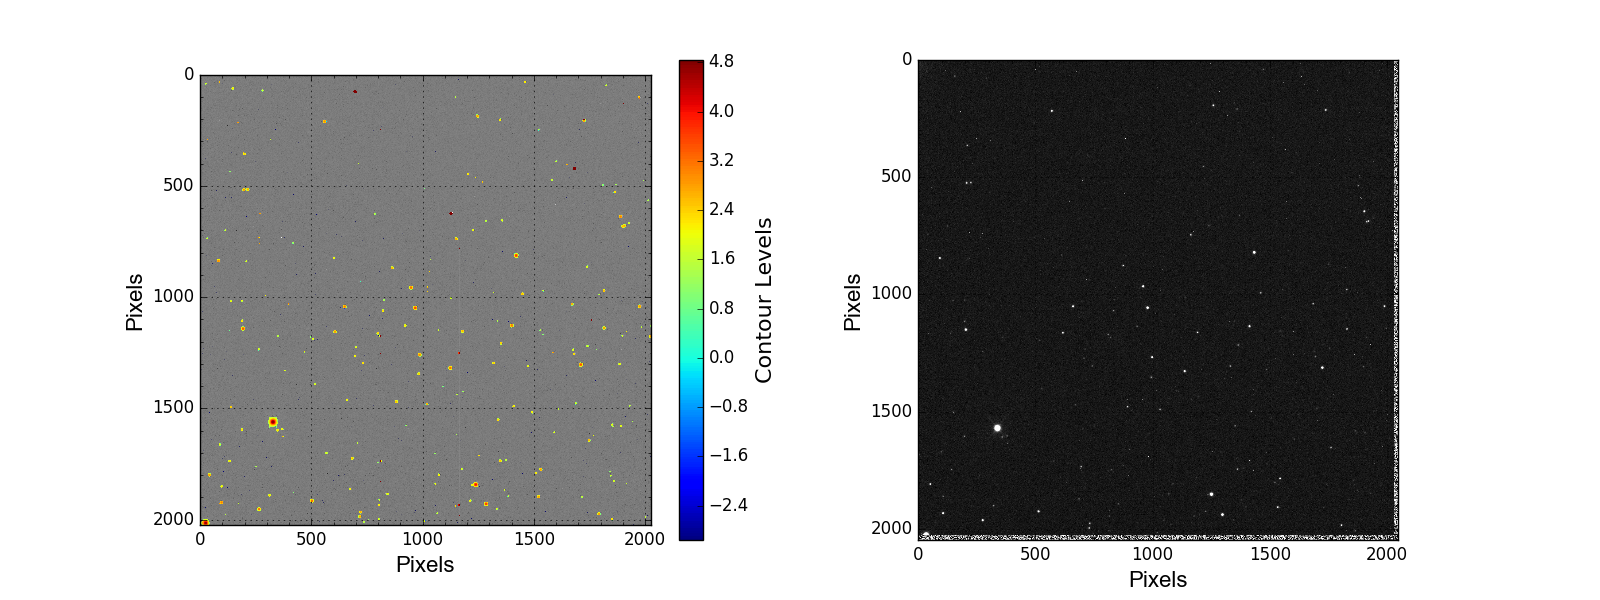
\includegraphics[scale=0.4]{compare.png}%\quad
  \caption{\textbf{Left:}\,Full reduced image that was provided. \textbf{Right:}\,Full corrected image. The corrected image was generated using a science image, darks, and flats. Both images were provided to show that image correction yielded the same full sky image that was already reduced.}
  \label{galaxy}
\end{figure*}

\begin{figure*}[ht]
  \centering
  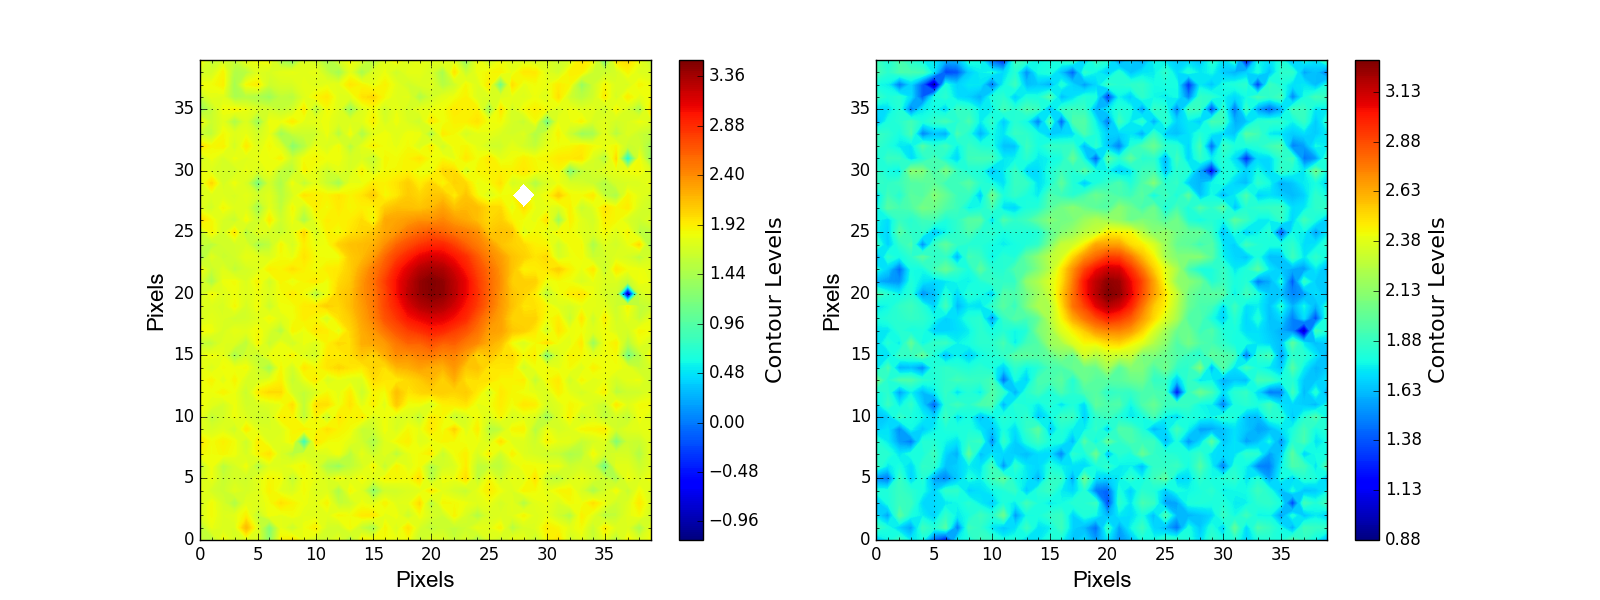
\includegraphics[scale=0.4]{stars.png}%\quad
  \caption{\textbf{Left:}\,The target, J-star, of the corrected image. \textbf{Right:}\,The reference/background star, J-standard, of the corrected image.}
  \label{star}
\end{figure*}

\floattable
\begin{deluxetable}{ccccCrlccc}
\tablecaption{Corrected Image Data \label{tab:mathmode}}
\tablecolumns{10}
%\tablenum{2}
\tablewidth{0pt}
\tablehead{
\colhead{Object} & \colhead{Date} & \colhead{Start} & \colhead{Full Sky} & \colhead{Background}& \colhead{Background} & \colhead{J$_\star$} & \colhead{J$_\dagger$}  & \colhead{Aperture} & \colhead{Magnitude} \\
\colhead{} & \colhead{} & \colhead{Time} & \colhead{Flux} & \colhead{Flux}& \colhead{Standard Deviation} & \colhead{Flux} & \colhead{Flux}  & \colhead{Size} & \colhead{} \\ }
\startdata
  J1614-1906 & 2014-06-07  & 14:51:40.337 & 65535.0 & 499885.161 & 19.00 &  171422.18  &  131921.58  & 40x40 & 13.22\\
\enddata
%\tablenotetext{a}{At exposure start.}
\tablecomments{Aperture photometry was done to generate the above data. Object, date, and start times were collected from the header information. Fluxes were collected by taking the sum of aperture regions and magnitudes were found using equation\,\ref{mageqn}.}
\label{imcortable}
\end{deluxetable}


%\indent Find if the star is a variable. Purpose of study.
%\section{Observations}

%\section{Apparatus}
%Telescope information and methods in header. Think about removal in final.

\section{Observation Planning}
\subsection{Signal to Noise}

The signal-to-noise is found for the star 16:41:15.8, +36:33:18, which has an R-mag of 14.27 and an I-mag of 13.84. Equation\,\ref{snr} is used with the resulting electron flux from aperture photometry of the centroid and reference star. The reference used is the star located at 16:41:23.587, +36:30:17.65. The reference star has an R-mag of 10.43 and an I-mag of 10.55. The star was observed with an exposure time of 43.002 seconds and RBI zero-points 21.00, 21.90, and 21.34, respectively. The signal-to-noise using equation\,\ref{snr} for a 43.002 second exposure time and bands RBI are 1102.06, 1010.02, and 1456.56, respectively. The flux is normalized to a second by dividing the photometry flux by the total exposure time, 43.002 seconds. The normalized signal to noise ratio, found by equation\,\ref{snr}, and the normalized flux yields ratios of 22.17, 22.20, and 31.59 for RBI filters, respectively. To reach a signal to noise ratio of 100, the exposure time required is 21 seconds. The resulting signal to noise ratios of each RBI filters with a 21 second exposure time are 101.59, 101.73, and 144.75, respectively.

\floattable
\begin{deluxetable}{ccccCrlc}
\tablecaption{Signal-to-noise table \label{tab:mathmode}}
\tablecolumns{8}
%\tablenum{2}
\tablewidth{0pt}
\tablehead{
\colhead{Star} & \colhead{B [u]} & \colhead{R [r]} & \colhead{I [i]} & \colhead{Flux/zp [R]} & \colhead{Flux/zp [B]} & \colhead{Flux/zp [I]} & \colhead{Exposure Time [s]} \\ }
\startdata
16:41:15.8, +36:33:18 & 15.17  & 14.27  & 13.84 & 491.46/21.00 & 492.85/21.90 &  997.79/21.34 & 43.002\\
\enddata
\tablecomments{The flux for each RBI filter, normalized to 1 second. The calculated zero points are also included in the table.}
\label{snrtable}
\end{deluxetable}

\clearpage
\subsection{Finder chart}

Table\,\ref{finderchart} was generated using the VizieR catalog. For the USNO-B 1.0 catalog the filter magnitudes are denoted with [2]. 

\floattable
\begin{deluxetable}{ccccCrlccc}
\tablecaption{Finder Chart \label{tab:mathmode}}
\tablecolumns{10}
%\tablenum{2}
\tablewidth{0pt}
\tablehead{
\colhead{Cluster} & \colhead{RA} & \colhead{Dec} & \colhead{RA (3rd)} & \colhead{Dec (3rd)} & \colhead{B (u)} & \colhead{V (g)} & \colhead{R (r)} & \colhead{I (i)} & \colhead{Catalog} \\ }
\startdata
  %Perseus & 3:18:36.774  & +41:30:54.55 &-& - & 18.95 &  -  &  16.71  & 15.16 & USNO-B 1.0\\
  %Train Wreck & 04:54:19  & +02:56:52.36 &-& - & - & -  & -  & 19.09  & USNO-B 1.0\\
  %Abell 569 & 07:09:10.138  & +48:37:14.45&-& - & 18.19 & - &  16.88 & - & GSC 2.2\\
  %Hydra & 10:36:50.55  & -27:31:42.06&-& - & 18.83 & - &  18.50 & 18.41 &USNO-B 1.0 \\
  %Coma & 12:59:48.67  & +27:58:57.47&-& - & - & -  & -  & 18.96 & USNO-B 1.0 \\
  %Abell 1689 & 13:11:18.453  & -01:18:39.54&-& -  & 17.32 & - &  16.11 & 15.75 & USNO-B 1.0\\
  Perseus* & 03:18:36.930 & 41:30:34.44 & 03:18:41.245 & 41:31:00.93 & 17.52(16.14) &  -  &  16.59(15.08)  & 16.35(14.86) & USNO-B 1.0\\
  Train Wreck* & 04:54:22.576  & 02:57:10:01 & 04:54:23.212 & 02:56:29.58 & 18.68(15.75) & -  & 18.32(14.86)  & (13.87)  & USNO-B 1.0\\
  Abell 569* & 07:09:10.138  & +48:37:14.45 & 07:09:03.906 & 48:36:54.44 & 18.68(15.11) & - &  18.32(14.64) & (14.27) & GSC 2.2\\
  Hydra* & 10:36:50.193  & -27:30:46.88 & 10:36:42.120 & -27:30:44.26 & 16.17(16.21) & - &  16.14(15.51) & 16.85(14.67) &USNO-B 1.0 \\
  Coma* & 12:59:46.936  & 27:59:30.87 & 12:59:43.718 & 27:59:40.75 & 16.05(11.62) & -  & 15.19(10.95)  & 14.87(11.05) & USNO-B 1.0 \\
  Abell 1689* & 13:11:30.0  & -01:20:17.0 & 13:11:22.862 & -01:17:36.08 & 17.32(17.47) & - &  16.11(15.69) & 15.75(15.69) & USNO-B 1.0\\
\enddata
%\tablenotetext{a}{At exposure start.}
\tablecomments{The data of these cluster members are found using the USNO-B 1.0 and GSC 2.2 catalogs. Both are found using the VizieR search tool\,(\url{http://vizier.u-strasbg.fr/viz-bin/VizieR-4}). The clusters denoted with (\*) were found by confirming with Aladin. The Aladin clusters also include measurements for a near bright objects. The BVRI magnitudes of the bright objects\,(3rd) are denoted after the cluster magnitude in the parenthesis.}
\label{finderchart}
\end{deluxetable}




Both figures\,\ref{galaxy} and \ref{star} were generated with the above photometry techniques. The image corrections and aperture photometry techniques specifically were used. To find the reference star, the Aladin full sky atlas was invoked\,(\url{http://aladin.u-strasbg.fr/AladinLite/}). The Aladin site allows for a quick look at bright objects and provides coordinate that can be plugged into VizieR for more accurate coordinates.

\begin{figure*}[ht]
  \centering
  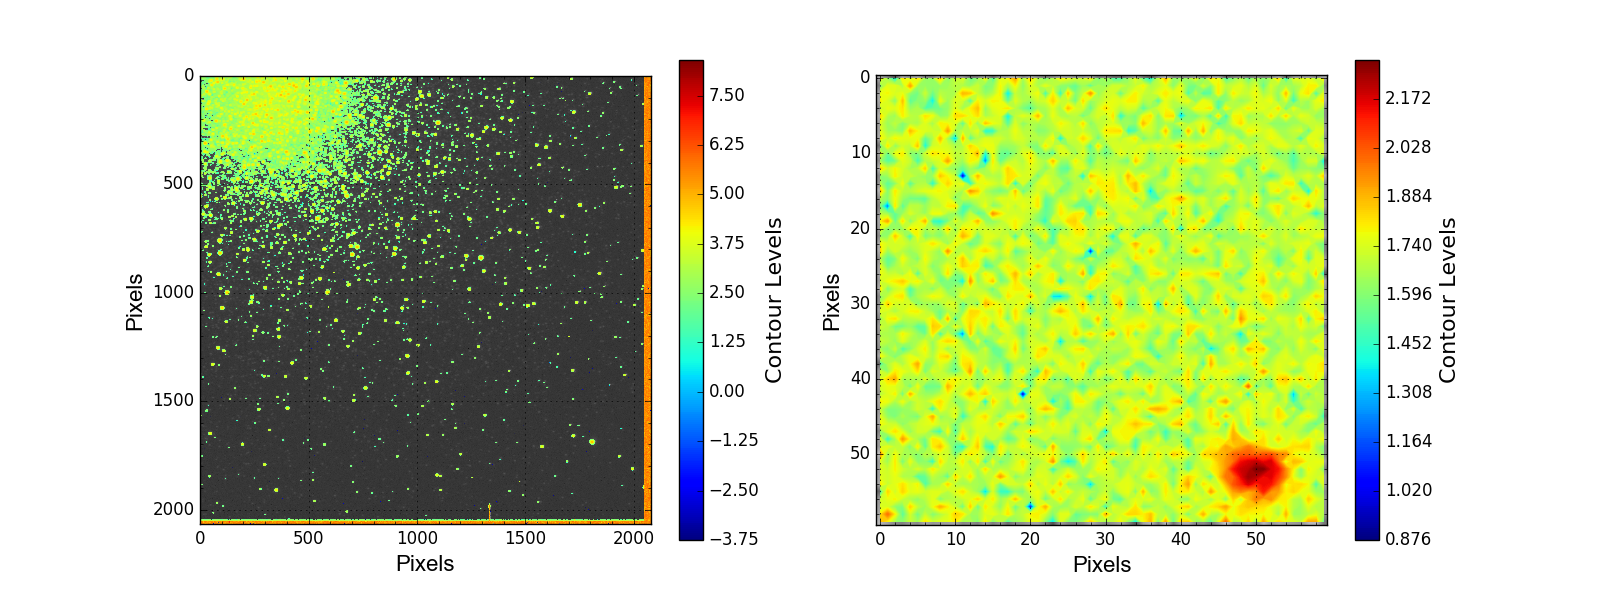
\includegraphics[scale=0.4]{galaxy.png}%\quad
  \caption{\textbf{Left:}\,Full image after corrections. \textbf{Right:}\,Background selection, note a slight intense region in the aperture, but it does not raise the standard deviation over the set threshold.}
  \label{galaxy}
\end{figure*}

\begin{figure*}[ht]
  \centering
  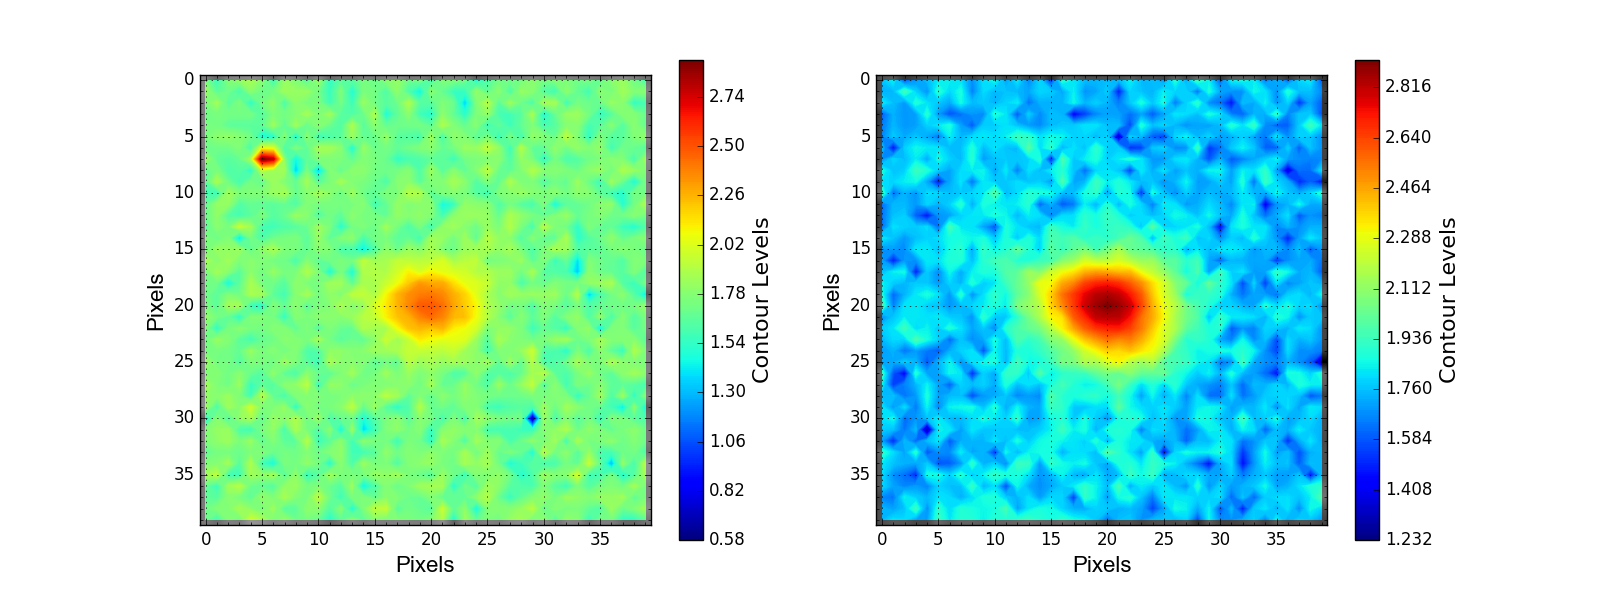
\includegraphics[scale=0.4]{star.png}%\quad
  \caption{\textbf{Left:}\,The target. \textbf{Right:}\,The reference/background star.}
  \label{star}
\end{figure*}

\subsection{Target availability}

The target availability for each cluster from table\,\ref{finderchart}. Each cluster is observed from Mauna Kea, which is located at 19.8261 $^\circ$N\,(latitude), -155.4708 $^\circ$E\,(azimuth). The rest of the needed parameters arise from target coordinates\,(RA/Dec) and the LST of the optimal transit period. The cluster is in a prime location higher than 30$^\circ$ above the horizon. The TEK detector on the UH 2.2\,m telescope is a 2048x2048 array of 0.22" pixels. The available filters are BVRI, although observation times are variable. The optimal observation time ranges are provided in table\,\ref{pointing}. Target availability curves were generated through equation\,\ref{elevation} with the corresponding parameters outlined in table\,\ref{targettable}. The elevation in degrees is plotted against the LST relative to midnight on LST.

\floattable
\begin{deluxetable}{ccccc}
\tablecaption{Target availability pointing times \label{tab:mathmode}}
\tablecolumns{5}
%\tablenum{2}
\tablewidth{0pt}
\tablehead{
\colhead{Cluster} & \colhead{Start Time}& \colhead{Start Time} & \colhead{End Time}& \colhead{End Time} \\
\colhead{} & \colhead{[hours off midnight]}& \colhead{[hh:mm:ss]} & \colhead{[hours off midnight]}& \colhead{[hh:mm:ss]} }
\startdata
Perseus & -6* & 18:00:00*  & 0.24 & 00:14:24\\
Train Wreck & -6* & 18:00:00* & 1.31 & 01:18:36\\
Abell 569 & -4.84* & 20:50:24* & 4 & 04:00:00 \\
Hydra & 0.53 & 00:31:48  & 5.59 & 05:35:24 \\
Coma & 1.06 & 01:03:36 & 6 & 06:00:00 \\
Abell 1689 & 1.81 & 01:48:36  & 6 & 06:00:00 \\
%2014-06-25  & 15:59:51  & lsc & 32613.693  $\pm$ 752.681 &  122060.992 $\pm$  809.923 & 14.933  $\pm$ 0.026\\
\enddata
%\tablenotetext{a}{At exposure start.}
\tablecomments{Observation times when the elevation is above 30$^\circ$ on Jan 18. The (*) and negative signs indicate times for the previous day (Jan 17).}
\label{pointing}
\end{deluxetable}

\floattable
\begin{deluxetable}{ccccCrlc}
\tablecaption{Target availability parameters \label{tab:mathmode}}
\tablecolumns{8}
%\tablenum{2}
\tablewidth{0pt}
\tablehead{
\colhead{Date} & \colhead{LST (midnight)} & \colhead{Elevation} & \colhead{Azimuth} & \colhead{RA} & \colhead{Dec} & \colhead{Latitude} & \colhead{Hour Angle} \\
\colhead{[mm-dd]} & \colhead{[hhmmsss]} & \colhead{} & \colhead{[0$^\circ$-360$^\circ$]}  & \colhead{[hh:mm:ss]} & \colhead{[dd:mm:ss]} & \colhead{[-90$^\circ$ - 90$^\circ$]} & \colhead{[Hours]}  }
\startdata
01-18 & 07h34m05.33s  & eqn\,\ref{elevation}  & -155.4708 & 13:11:30 & -01:20:17 &  19.8261 & eqn\,\ref{hourangle}\\
%2014-06-25  & 15:59:51  & lsc & 32613.693  $\pm$ 752.681 &  122060.992 $\pm$  809.923 & 14.933  $\pm$ 0.026\\
\enddata
%\tablenotetext{a}{At exposure start.}
\tablecomments{Negative azimuth angles are subtracted from 360 to result in a positive angle.}
\label{targettable}
\end{deluxetable}


\begin{figure*}[ht]
  \centering
  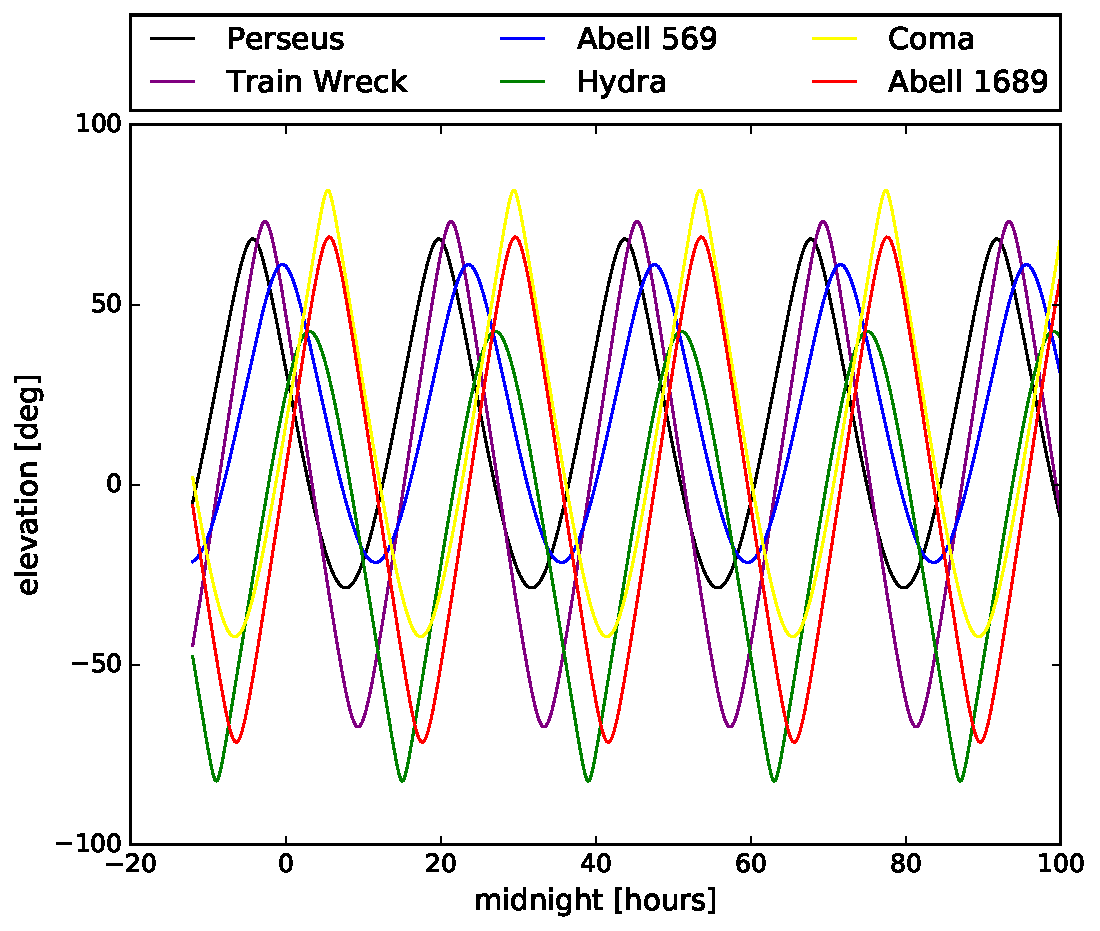
\includegraphics[scale=0.4]{azimuth.pdf}%\quad
  \caption{Target availabilities for all six clusters mentioned in table\,\ref{finderchart}. The elevation starts at 30$^\circ$ from delta\_midnight hours from -6 to 6.}
  \label{targetavail}
\end{figure*}


\clearpage
\subsection{Field of view}
The field of view is shown for the Abell 1689 region, represented in figure\,\ref{fov}. The objects within the field of view with the coordinates based off of the purple cross. Bright points were chosen based off of the field of view and confirmed with the VizieR catalog.

\begin{figure*}[ht]
  \centering
  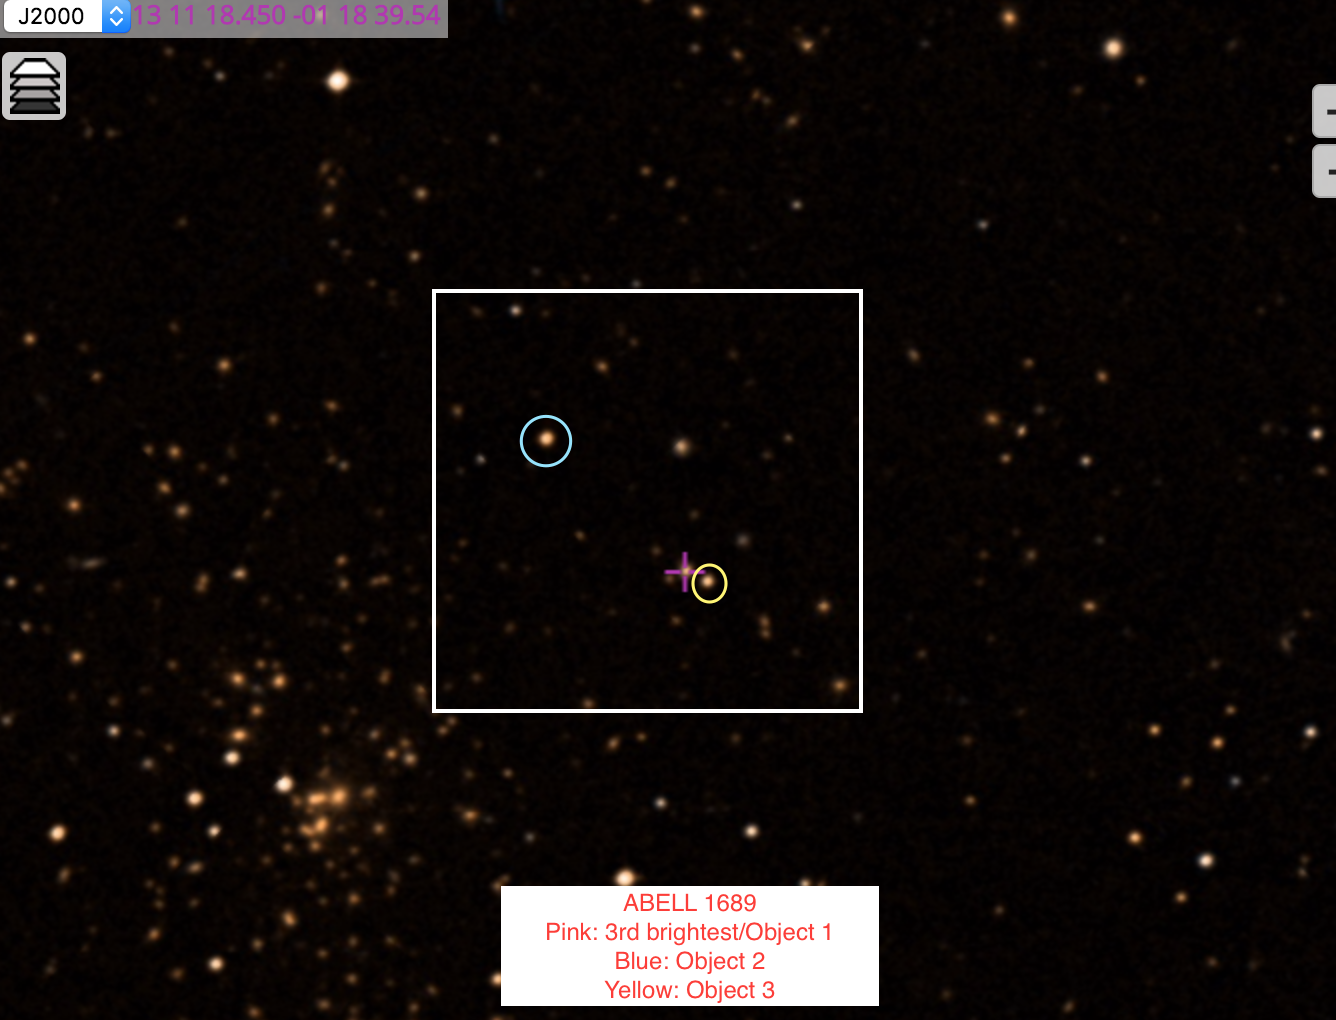
\includegraphics[scale=0.3]{aladin.png}%\quad
  \caption{A sample magnified field of view from the Aladin full sky atlas. This field of view is of Abell 1689, where the coordinates are as labeled.}
  \label{fov}
\end{figure*}


%\acknowledgments
\clearpage
\section{Appendix}
Source code of the python scripts to conduct photometry and to generate target availabilities are included.
\\
\noindent 1) azimuth.py - Generates elevation plots regarding target availability.
\\
2) decgalax.py - Photometry script, produces flux and magnitudes of aperture photometry.
\\
3) dark.py - Image correction script, to generate corrected images using flats, darks, and corrected images.


%\vspace{5mm}
%
%\begin{thebibliography}{}
%
%
%\bibitem[Cody et al.(2014)]{2}
%Cody et al., 2014, Astronomical Journal, volume 147, p. 82
%
%\bibitem[Herbst(2012)]{5}
%Herbst, W. 2012, Journal of the American Association of Variable Star Observers, 40, 448
%
%\bibitem[Gham et al.(1995)]{6}
%Gahm, G. F., Loden. K. Gullbring, E., \& Hartstein, D. 1995, A\&A, 301, 89 
%
%\bibitem[Matthews(2012)]{4}
%Mathews, G. S., Williams, J. P., \& Menard, F. 2012, ´ ApJ, 753, 59
%
%\bibitem[Preibisch(2008)]{3}
%Preibisch \& Mamajek, 2008, from the book Handbook of Star Forming Regions, Volume II, ed. B. Reipurth.
%
%
%
%\bibitem[Snow(1984)]{1}
%Snow, Theodore P., and Theodore P. Snow. Essentials of the Dynamic Universe: An Introduction to Astronomy. St. Paul: West, 1984. Print.
%
%
%\end{thebibliography}




%% Appendix material should be preceded with a single \appendix command.
%% There should be a \section command for each appendix. Mark appendix
%% subsections with the same markup you use in the main body of the paper.

%% Each Appendix (indicated with \section) will be lettered A, B, C, etc.
%% The equation counter will reset when it encounters the \appendix
%% command and will number appendix equations (A1), (A2), etc.


%% The reference list follows the main body and any appendices.
%% Use LaTeX's thebibliography environment to mark up your reference list.
%% Note \begin{thebibliography} is followed by an empty set of
%% curly braces.  If you forget this, LaTeX will generate the error
%% "Perhaps a missing \item?".
%%
%% thebibliography produces citations in the text using \bibitem-\cite
%% cross-referencing. Each reference is preceded by a
%% \bibitem command that defines in curly braces the KEY that corresponds
%% to the KEY in the \cite commands (see the first section above).
%% Make sure that you provide a unique KEY for every \bibitem or else the
%% paper will not LaTeX. The square brackets should contain
%% the citation text that LaTeX will insert in
%% place of the \cite commands.

%% We have used macros to produce journal name abbreviations.
%% \aastex provides a number of these for the more frequently-cited journals.
%% See the Author Guide for a list of them.

%% Note that the style of the \bibitem labels (in []) is slightly
%% different from previous examples.  The natbib system solves a host
%% of citation expression problems, but it is necessary to clearly
%% delimit the year from the author name used in the citation.
%% See the natbib documentation for more details and options.


\end{document}

%% End of file `sample.tex'.
